%% Creator: Inkscape inkscape 0.92.5, www.inkscape.org
%% PDF/EPS/PS + LaTeX output extension by Johan Engelen, 2010
%% Accompanies image file 'DynamicsWT1DOF_Blade.pdf' (pdf, eps, ps)
%%
%% To include the image in your LaTeX document, write
%%   \input{<filename>.pdf_tex}
%%  instead of
%%   \includegraphics{<filename>.pdf}
%% To scale the image, write
%%   \def\svgwidth{<desired width>}
%%   \input{<filename>.pdf_tex}
%%  instead of
%%   \includegraphics[width=<desired width>]{<filename>.pdf}
%%
%% Images with a different path to the parent latex file can
%% be accessed with the `import' package (which may need to be
%% installed) using
%%   \usepackage{import}
%% in the preamble, and then including the image with
%%   \import{<path to file>}{<filename>.pdf_tex}
%% Alternatively, one can specify
%%   \graphicspath{{<path to file>/}}
%% 
%% For more information, please see info/svg-inkscape on CTAN:
%%   http://tug.ctan.org/tex-archive/info/svg-inkscape
%%
\begingroup%
  \makeatletter%
  \providecommand\color[2][]{%
    \errmessage{(Inkscape) Color is used for the text in Inkscape, but the package 'color.sty' is not loaded}%
    \renewcommand\color[2][]{}%
  }%
  \providecommand\transparent[1]{%
    \errmessage{(Inkscape) Transparency is used (non-zero) for the text in Inkscape, but the package 'transparent.sty' is not loaded}%
    \renewcommand\transparent[1]{}%
  }%
  \providecommand\rotatebox[2]{#2}%
  \newcommand*\fsize{\dimexpr\f@size pt\relax}%
  \newcommand*\lineheight[1]{\fontsize{\fsize}{#1\fsize}\selectfont}%
  \ifx\svgwidth\undefined%
    \setlength{\unitlength}{330.2050992bp}%
    \ifx\svgscale\undefined%
      \relax%
    \else%
      \setlength{\unitlength}{\unitlength * \real{\svgscale}}%
    \fi%
  \else%
    \setlength{\unitlength}{\svgwidth}%
  \fi%
  \global\let\svgwidth\undefined%
  \global\let\svgscale\undefined%
  \makeatother%
  \begin{picture}(1,0.58394422)%
    \lineheight{1}%
    \setlength\tabcolsep{0pt}%
    \put(0,0){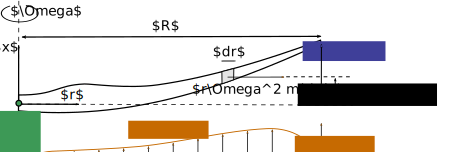
\includegraphics[width=\unitlength,page=1]{DynamicsWT1DOF_Blade.pdf}}%
    \put(0.12402166,0.54612802){\color[rgb]{0,0,0}\makebox(0,0)[t]{\lineheight{0}\smash{\begin{tabular}[t]{c}$\Omega$\end{tabular}}}}%
    \put(0.02580057,0.45881309){\color[rgb]{0,0,0}\makebox(0,0)[t]{\lineheight{0}\smash{\begin{tabular}[t]{c}$x$\end{tabular}}}}%
    \put(0,0){\includegraphics[width=\unitlength,page=2]{DynamicsWT1DOF_Blade.pdf}}%
    \put(0.41475476,0.51027288){\color[rgb]{0,0,0}\makebox(0,0)[t]{\lineheight{0}\smash{\begin{tabular}[t]{c}$R$\end{tabular}}}}%
    \put(0.19220149,0.34743672){\color[rgb]{0,0,0}\makebox(0,0)[t]{\lineheight{0}\smash{\begin{tabular}[t]{c}$r$\end{tabular}}}}%
    \put(0,0){\includegraphics[width=\unitlength,page=3]{DynamicsWT1DOF_Blade.pdf}}%
    \put(0.73971697,0.38120182){\color[rgb]{0,0,0}\makebox(0,0)[lt]{\begin{minipage}{0.33821158\unitlength}\centering $\Phi(r)q(t)$\end{minipage}}}%
    \put(0,0){\includegraphics[width=\unitlength,page=4]{DynamicsWT1DOF_Blade.pdf}}%
    \put(0.66146945,0.35604199){\color[rgb]{0,0,0}\makebox(0,0)[t]{\lineheight{0}\smash{\begin{tabular}[t]{c}$r\Omega^2 m(r) dr$\end{tabular}}}}%
    \put(0,0){\includegraphics[width=\unitlength,page=5]{DynamicsWT1DOF_Blade.pdf}}%
    \put(0.5690054,0.44746184){\color[rgb]{0,0,0}\makebox(0,0)[t]{\lineheight{0}\smash{\begin{tabular}[t]{c}$dr$\end{tabular}}}}%
    \put(0,0){\includegraphics[width=\unitlength,page=6]{DynamicsWT1DOF_Blade.pdf}}%
    \put(0.32344218,0.29073343){\color[rgb]{0.77647059,0.41568627,0.00392157}\makebox(0,0)[lt]{\begin{minipage}{0.19508645\unitlength}\centering $p_x(r,t)$ \end{minipage}}}%
    \put(0,0){\includegraphics[width=\unitlength,page=7]{DynamicsWT1DOF_Blade.pdf}}%
    \put(0.72801481,0.25387236){\color[rgb]{0.77647059,0.41568627,0.00392157}\makebox(0,0)[lt]{\begin{minipage}{0.19395523\unitlength}\centering $f_{e}$ \end{minipage}}}%
    \put(0,0){\includegraphics[width=\unitlength,page=8]{DynamicsWT1DOF_Blade.pdf}}%
    \put(-0.0243134,0.3145387){\color[rgb]{0.23921569,0.6,0.3372549}\makebox(0,0)[lt]{\begin{minipage}{0.13514515\unitlength}\centering B\end{minipage}}}%
    \put(-0.54833275,3.10038802){\color[rgb]{0,0,0}\makebox(0,0)[lt]{\begin{minipage}{0.11248419\unitlength}\centering \end{minipage}}}%
    \put(0.74707494,0.4838035){\color[rgb]{0.24705882,0.24705882,0.6}\makebox(0,0)[lt]{\begin{minipage}{0.20115388\unitlength}\centering $q(t)$\end{minipage}}}%
    \put(0,0){\includegraphics[width=\unitlength,page=9]{DynamicsWT1DOF_Blade.pdf}}%
    \put(0.8177364,0.06063316){\color[rgb]{0,0,0}\makebox(0,0)[t]{\lineheight{0}\smash{\begin{tabular}[t]{c}$1$\end{tabular}}}}%
    \put(0.30510872,0.08528395){\color[rgb]{0,0,0}\makebox(0,0)[lt]{\begin{minipage}{0.33821158\unitlength}\centering $\Phi(r)$\end{minipage}}}%
    \put(0.0303432,0.14885425){\color[rgb]{0,0,0}\makebox(0,0)[t]{\lineheight{0}\smash{\begin{tabular}[t]{c}$x$\end{tabular}}}}%
    \put(0.18379193,0.03629903){\color[rgb]{0,0,0}\makebox(0,0)[t]{\lineheight{0}\smash{\begin{tabular}[t]{c}$r$\end{tabular}}}}%
    \put(0,0){\includegraphics[width=\unitlength,page=10]{DynamicsWT1DOF_Blade.pdf}}%
  \end{picture}%
\endgroup%
